% Host wiring: M1-A/B/C internals are separate module-detail diagrams.
\documentclass[tikz,border=0pt]{standalone}
\usepackage[T1]{fontenc}
\usepackage[american]{circuitikz}
\usetikzlibrary{arrows.meta,backgrounds,fit}
\definecolor{MainBus}{HTML}{9C2F24}
\definecolor{SenseWire}{HTML}{1769AA}
\definecolor{SdaWire}{HTML}{00838F}
\definecolor{SclWire}{HTML}{6A4C93}
\definecolor{LogicPower}{HTML}{B05A00}
\definecolor{ModuleFill}{HTML}{F4F7FA}
\tikzset{
  power/.style={draw=LogicPower,line width=1pt},
  main/.style={draw=MainBus,line width=2pt},
  sense/.style={draw=SenseWire,line width=1pt},
  sda/.style={draw=SdaWire,line width=1pt},
  scl/.style={draw=SclWire,line width=1pt},
  body/.style={draw=black!65,fill=ModuleFill,rounded corners=2pt,line width=.8pt},
  title/.style={font=\sffamily\bfseries,align=center},
  note/.style={font=\sffamily\scriptsize,align=center},
  pin/.style={font=\sffamily\tiny,inner sep=2pt},
  net/.style={font=\sffamily\scriptsize\bfseries,inner sep=2pt,fill=white}
}
\newcommand{\Port}[3]{\filldraw[fill=white,draw=black!70] (#1) circle (2pt);\node[pin,anchor=#2] at (#1) {#3};}
% Vertical wire bridge: crossing without an electrical junction.
\newcommand{\Bridge}[3]{%
  \draw[white,line width=4pt] (#1,#2+.15) -- (#1,#2-.15);
  \draw[white,line width=4pt] (#1,#2+.15)
    .. controls (#1+.22,#2+.10) and (#1+.22,#2-.10) .. (#1,#2-.15);
  \draw[draw=#3,line width=1pt] (#1,#2+.15)
    .. controls (#1+.22,#2+.10) and (#1+.22,#2-.10) .. (#1,#2-.15);
}
\begin{document}
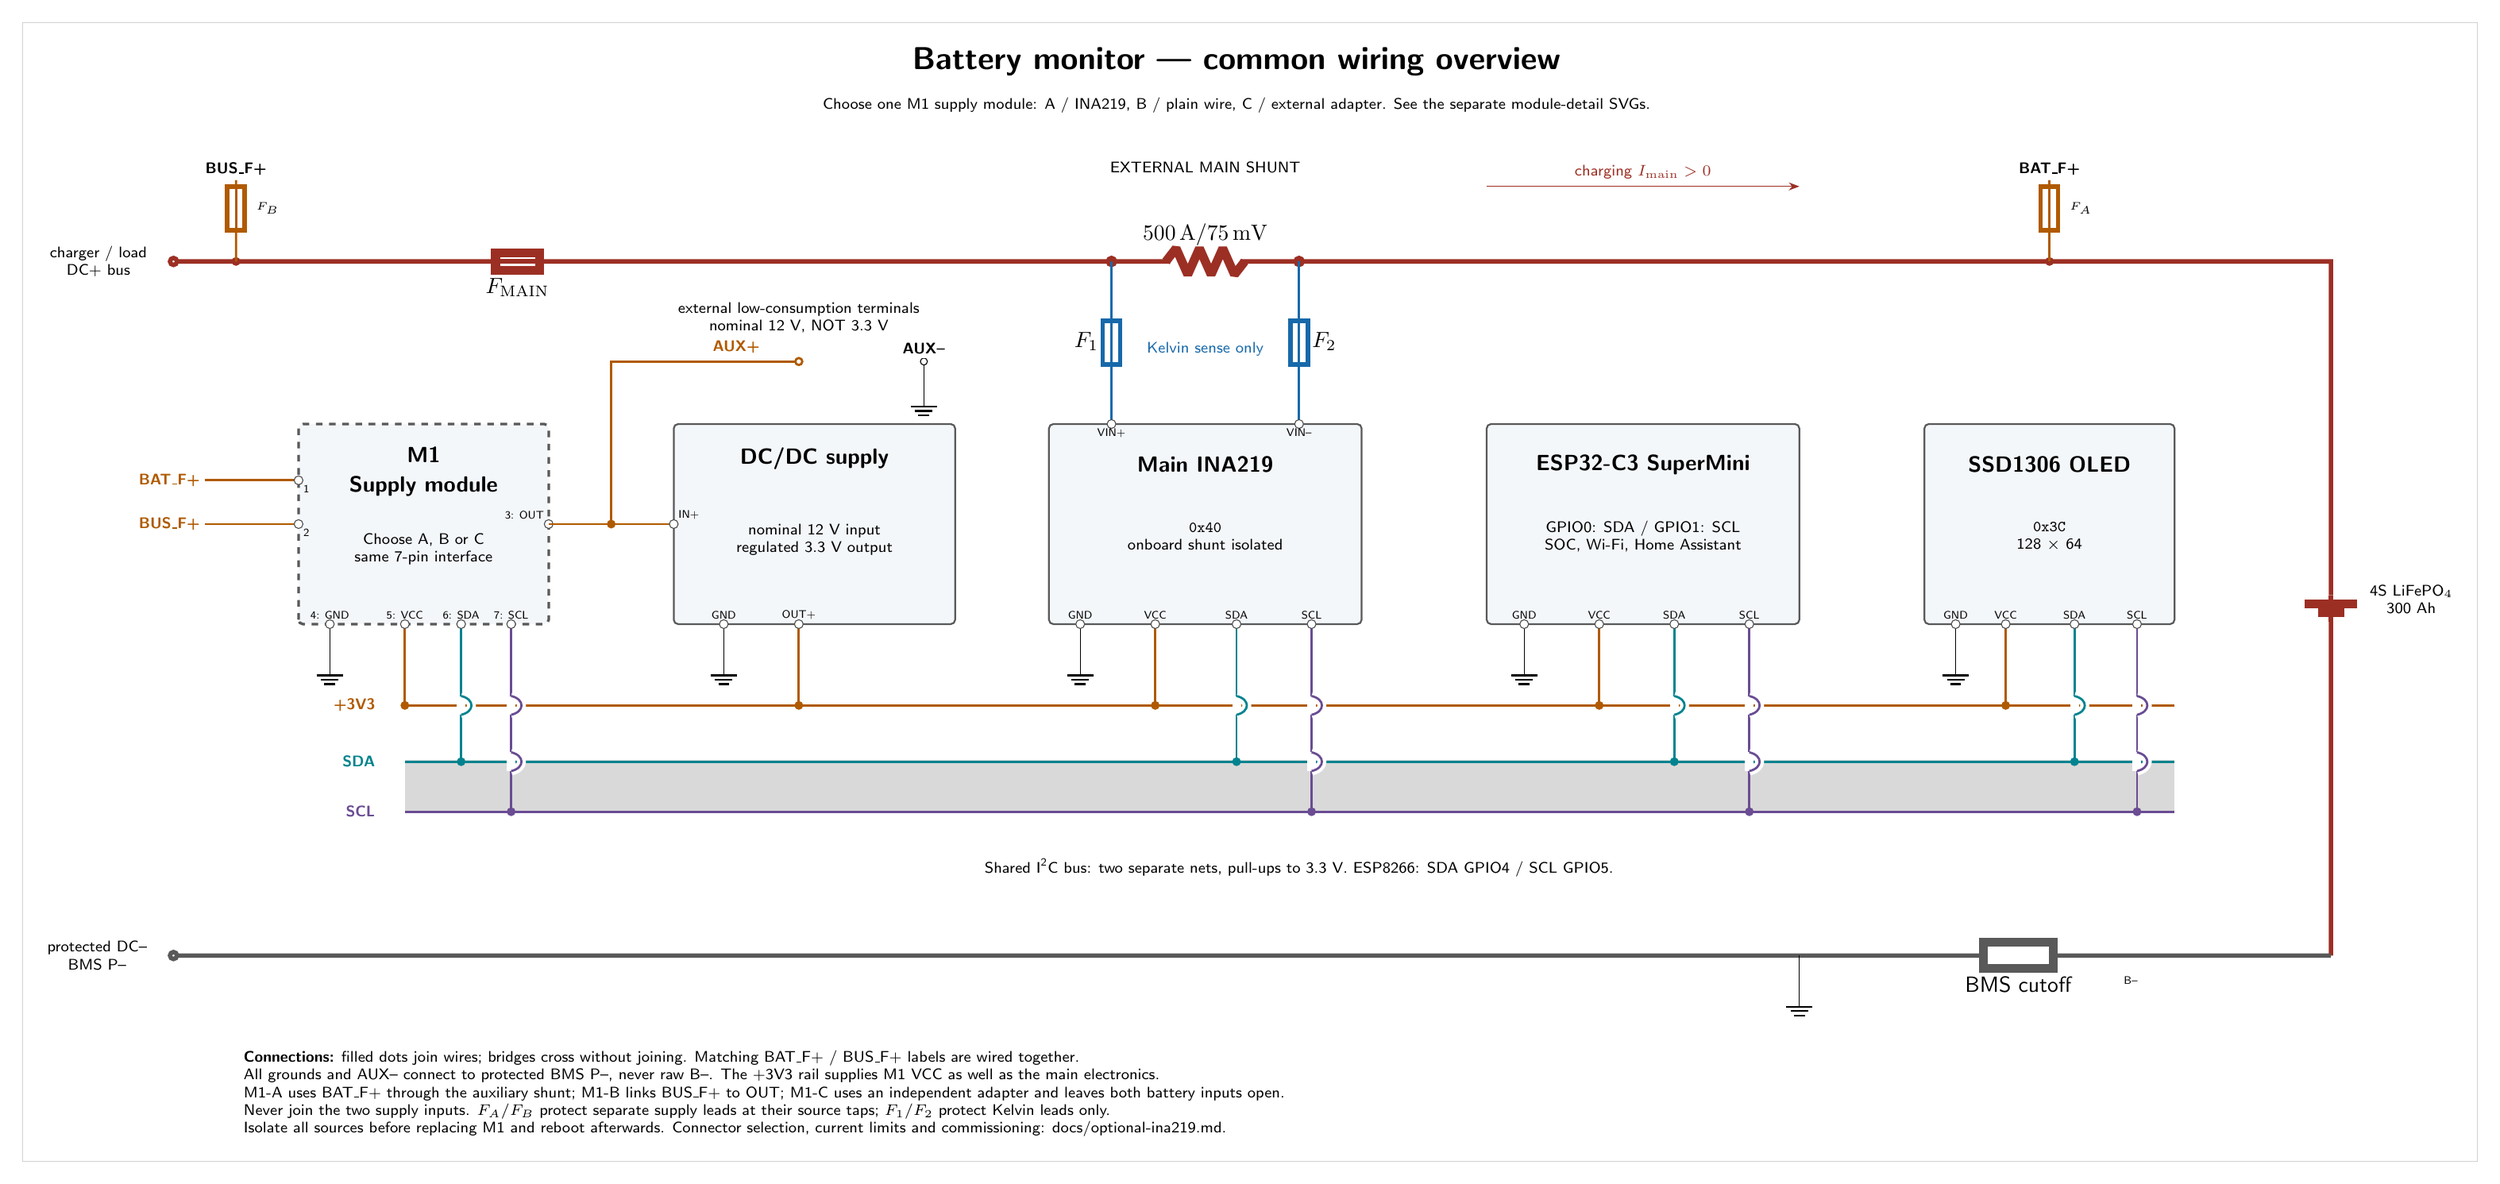
\begin{tikzpicture}[font=\sffamily]
\begin{scope}[local bounding box=diagram-content]
  \node[title,font=\sffamily\Large\bfseries] at (15,15) {Battery monitor --- common wiring overview};
  \node[note] at (15,14.3) {Choose one M1 supply module: A / INA219, B / plain wire, C / external adapter. See the separate module-detail SVGs.};

  % Original orientation, with the external shunt above its main INA219.
  \draw[main] (-2,11.8) node[ocirc] {} -- (2,11.8)
    to[fuse,l_={$F_{\rm MAIN}$}] (5,11.8) -- (13,11.8)
    to[R,l^={$500\,\mathrm{A}/75\,\mathrm{mV}$},*-*] (16,11.8)
    -- (32.5,11.8) to[battery1] (32.5,.7);
  \draw[draw=black!65,line width=2pt] (32.5,.7) -- (29,.7)
    to[generic,l^={BMS cutoff}] (26,.7) -- (-2,.7) node[ocirc] {};
  \node[note,anchor=east] at (-2.3,11.8) {charger / load\\DC+ bus};
  \node[note,anchor=east] at (-2.3,.7) {protected DC--\\BMS P--};
  \node[note,anchor=west] at (33,6.4) {4S LiFePO$_4$\\300 Ah};
  \node[pin] at (29.3,.3) {B--};
  \draw (24,.7) -- (24,.3) node[ground] {};
  \node[note] at (14.5,13.3) {EXTERNAL MAIN SHUNT};
  \draw[-{Stealth},MainBus] (19,13) -- (24,13)
    node[midway,above,note] {charging $I_{\rm main}>0$};

  % Named supply feeds keep the long battery-side lead away from Kelvin wiring.
  \fill[MainBus] (-1,11.8) circle (2pt);
  \draw[power] (-1,11.8) -- (-1,12.2) to[fuse] (-1,13.1);
  \node[net,anchor=south] at (-1,13.1) {BUS\_F+};
  \node[pin,anchor=west] at (-.75,12.65) {$F_B$};
  \fill[MainBus] (28,11.8) circle (2pt);
  \draw[power] (28,11.8) -- (28,12.2) to[fuse] (28,13.1);
  \node[net,anchor=south] at (28,13.1) {BAT\_F+};
  \node[pin,anchor=west] at (28.25,12.65) {$F_A$};
  \draw[sense] (13,11.8) to[fuse,l_={$F_1$}] (13,9.2);
  \draw[sense] (16,11.8) to[fuse,l={$F_2$}] (16,9.2);
  \node[note,text=SenseWire] at (14.5,10.4) {Kelvin sense only};

  % Supply module and DC/DC sit in the same row as the controller/sensors.
  \draw[body,dashed,line width=1.2pt] (0,6) rectangle (4,9.2);
  \node[title] at (2,8.7) {M1};
  \node[title] at (2,8.2) {Supply module};
  \node[note] at (2,7.2) {Choose A, B or C\\same 7-pin interface};
  \draw[power] (-1.5,8.3) -- (0,8.3);
  \draw[power] (-1.5,7.6) -- (0,7.6);
  \node[net,anchor=east,text=LogicPower] at (-1.5,8.3) {BAT\_F+};
  \node[net,anchor=east,text=LogicPower] at (-1.5,7.6) {BUS\_F+};
  \Port{0,8.3}{north west}{1}
  \Port{0,7.6}{north west}{2}
  \Port{4,7.6}{south east}{3: OUT}

  \draw[body] (6,6) rectangle (10.5,9.2);
  \node[title] at (8.25,8.65) {DC/DC supply};
  \node[note] at (8.25,7.35) {nominal 12 V input\\regulated 3.3 V output};
  \draw[power] (4,7.6) -- (6,7.6);
  \Port{6,7.6}{south west}{IN+}
  % AUX+ branches before the converter and also supplies external small loads.
  \fill[LogicPower] (5,7.6) circle (2pt);
  \draw[power] (5,7.6) -- (5,10.2) -- (8,10.2) node[ocirc] {};
  \node[net,anchor=south,text=LogicPower] at (7,10.25) {AUX+};
  \draw (10,10.2) node[ocirc] {} -- (10,9.9) node[ground] {};
  \node[net,anchor=south] at (10,10.25) {AUX--};
  \node[note] at (8,10.9) {external low-consumption terminals\\nominal 12 V, NOT 3.3 V};

  \draw[body] (12,6) rectangle (17,9.2);
  \node[title] at (14.5,8.55) {Main INA219};
  \node[note] at (14.5,7.4) {\texttt{0x40}\\onboard shunt isolated};
  \Port{13,9.2}{north}{VIN+}
  \Port{16,9.2}{north}{VIN--}
  \draw[body] (19,6) rectangle (24,9.2);
  \node[title] at (21.5,8.55) {ESP32-C3 SuperMini};
  \node[note] at (21.5,7.4) {GPIO0: SDA / GPIO1: SCL\\SOC, Wi-Fi, Home Assistant};
  \draw[body] (26,6) rectangle (30,9.2);
  \node[title] at (28,8.55) {SSD1306 OLED};
  \node[note] at (28,7.4) {\texttt{0x3C}\\128 $\times$ 64};

  % All logic and data contacts face the three continuous shared rails.
  \foreach \x/\label in {.5/{4: GND},6.8/{GND},12.5/{GND},19.6/{GND},26.5/{GND}} {
    \draw (\x,6) -- (\x,5.6) node[ground] {};
    \Port{\x,6}{south}{\label}
  }
  \draw[power] (1.7,4.7) -- (30,4.7);
  \node[net,anchor=east,text=LogicPower] at (1.3,4.7) {+3V3};
  \foreach \x/\label in {1.7/{5: VCC},8/{OUT+},13.7/{VCC},20.8/{VCC},27.3/{VCC}} {
    \draw[power] (\x,6) -- (\x,4.7);
    \fill[LogicPower] (\x,4.7) circle (2pt);
    \Port{\x,6}{south}{\label}
  }
  % Two separate I2C conductors share a subtle gray cable jacket.
  \draw[black!15,line width=24pt] (1.7,3.4) -- (30,3.4);
  \draw[sda] (1.7,3.8) -- (30,3.8);
  \draw[scl] (1.7,3) -- (30,3);
  \node[net,anchor=east,text=SdaWire] at (1.3,3.8) {SDA};
  \node[net,anchor=east,text=SclWire] at (1.3,3) {SCL};
  \foreach \x/\label in {2.6/{6: SDA},15/{SDA},22/{SDA},28.4/{SDA}} {
    \draw[sda] (\x,6) -- (\x,3.8);
    \Bridge{\x}{4.7}{SdaWire}
    \fill[SdaWire] (\x,3.8) circle (2pt);
    \Port{\x,6}{south}{\label}
  }
  \foreach \x/\label in {3.4/{7: SCL},16.2/{SCL},23.2/{SCL},29.4/{SCL}} {
    \draw[scl] (\x,6) -- (\x,3);
    \Bridge{\x}{4.7}{SclWire}
    \Bridge{\x}{3.8}{SclWire}
    \fill[SclWire] (\x,3) circle (2pt);
    \Port{\x,6}{south}{\label}
  }
  \node[note] at (16,2.1) {Shared I\textsuperscript{2}C bus: two separate nets, pull-ups to 3.3 V. ESP8266: SDA GPIO4 / SCL GPIO5.};

  \node[note,align=left,anchor=north west] at (-1,-.7)
    {\textbf{Connections:} filled dots join wires; bridges cross without joining. Matching BAT\_F+ / BUS\_F+ labels are wired together.\\
     All grounds and AUX-- connect to protected BMS P--, never raw B--. The +3V3 rail supplies M1 VCC as well as the main electronics.\\
     M1-A uses BAT\_F+ through the auxiliary shunt; M1-B links BUS\_F+ to OUT; M1-C uses an independent adapter and leaves both battery inputs open.\\
     Never join the two supply inputs. $F_A/F_B$ protect separate supply leads at their source taps; $F_1/F_2$ protect Kelvin leads only.\\
     Isolate all sources before replacing M1 and reboot afterwards. Connector selection, current limits and commissioning: docs/optional-ina219.md.};
\end{scope}
\begin{scope}[on background layer]
  \node[fill=white,draw=black!18,fit=(diagram-content),inner sep=8pt] {};
\end{scope}
\end{tikzpicture}
\end{document}
